\documentclass[acmtog]{acmart}
\usepackage{graphicx}
\usepackage{subfigure}
\usepackage{natbib}
\usepackage{listings}
\usepackage{bm}
\usepackage{amsmath}

\definecolor{blve}{rgb}{0.3372549 , 0.61176471, 0.83921569}
\definecolor{gr33n}{rgb}{0.29019608, 0.7372549, 0.64705882}
\makeatletter
\lst@InstallKeywords k{class}{classstyle}\slshape{classstyle}{}ld
\makeatother
\lstset{language=C++,
	basicstyle=\ttfamily,
	keywordstyle=\color{blve}\ttfamily,
	stringstyle=\color{red}\ttfamily,
	commentstyle=\color{magenta}\ttfamily,
	morecomment=[l][\color{magenta}]{\#},
	classstyle = \bfseries\color{gr33n}, 
	tabsize=2
}
\lstset{basicstyle=\ttfamily}

% Title portion
\title{Assignment 3: {Ray Tracing Basics}} 

\author{Name:\quad ZhouShouchen  \\ student number:\ 2021533042
\\email:\quad zhoushch@shanghaitech.edu.cn}
\setlength{\headheight}{25pt}

% Document starts
\begin{document}
\maketitle

\vspace*{2 ex}

\section{Introduction}
In this assignment, the following tasks are finished by using ray-tracing.
\begin{itemize}
\item Task1: generate rays from camera
\item Task2: ray geometry intersection
\item Task3: Phong lighting at intersection
\item Task4: light ray sampling for soft shadow
\item Task5: anti-aliasing by super-resolution
\item Bonus1: texture mapping
\item Bonus2: normal/displacement texture
\item Bonus3: advanced anti-aliasing
\end{itemize}

\section{Implementation Details}
Briefly introduct the ray tracing.\\
for each pixel of the image, we can generate a ray from the camera, and that ray will intersect with an object or a light.\\
if it is a light, the color of the pixel is just the light's color,
otherwise, the intersection point can be beam by lights, and we can calculate its light imformations with phong lightning model.\\
and when dealing the problem, we may face jaggies, and we can solve it by anti-aliasing.\\
we also need to generate shadows, which can be solved by Task4: light ray sampling for soft shadow.\\
And the details are as followed.

\subsection{generate rays from camera}
to generate a ray from camera, we need to set the parameter of the camera first.\\
with the position of the camera, and the point the camera is looking at, we cna calculate the vectors of the camera:\\
$forword = look\_at - position, right = forword \times ref-up, $\\ $up = right \times forword$\\
and all these vectors should be normalized.\\
after setting the parameters, we can generate rays from the camera.\\
for the starter(without anti-aliasing), we just need to generate one ray with each pixel, which means that the ray is generate from the camera, and pointing to the center of a pixel's center.\\
so one important thing is to transfrom the coordinate of the piexl's center from screen space to the world space.\\
suppose that the scene's coordinate is $(dx,dy)$,\\
the scene's center's world space coordinate is $screen\_center = position + focal\_len * forward$\\
with these two vectors, we can calculate the world coordinate by 
$world\_coord = screen\_center$\\
              $+ ((2 * dx / width - 1) * ratio * focal\_len * tan(fov * PI / 180 / 2)) * right$\\
              $+ ((2 * dy / height - 1) * focal\_len * tan(fov * PI / 180 / 2) * focal\_len) * up$\\
and then we can easily generate the ray which start at the camera's position, pointing to the $world\_coord$

\subsection{ray geometry intersection}
for this assignment, we just need to consider three types of intersection.\\
to story the imformations of the intersection, we need to story the following thigns:\\
the type of the intersection point: initially it is $NONE$, if it is interacted with light, modify it into $LIGHT$, with an object, modify into $GEOMETRY$\\
and the position, normal vector of the intersection point\\
and the distence between the camera and the intersection point, because of we need to take the first intersection point along one ray.\\
the detail of how to judge whether it is interacted with different geometry shapes:\\
and if we calculate a $t$, we need to check whether the $t$ is in the range of the ray $[t\_min,t\_max]$
\begin{itemize}
	\item triangle
		\\
		suppose that the three vertices of the triangle are $v_0, v_1, v_2$\\
		and the intersection point $o + td = b_1v_1 + b_2v_2 + (1 - b_1 - b_2)v_0$\\
		so $td + (v_0-v_1)b_1 + (v_0-v_2)b_2 = v_0 - o$\\
		with Cramer's Rule, we can solve the equation above by letting\\
		$e_1 = v_1 - v_0, e_2 = v_2 - v_0, s = o - v_0, s_1 = d \times e_2, s_2 = s \times e_1$\\
		so $t = \frac{s_2 \cdot e_2}{s_1\cdot e_1}, b_1 = \frac{s_1 \cdot s}{s_1 \cdot e_1} , b_2 = \frac{s_2 \cdot d}{s_1 \cdot e_1}$\\
		if $b_1, b_2, 1 - b_1 - b_2$ is all in range $[0,1]$\\
		then we can say that the ray is intersected with the triangle.
		and we can easily use the cross to calculate the normal vector $\vec{normal} = (v_1 - v_0) \times (v_2 - v_1)$

	\item rectangle
		\\
		we have the center of the rectangle, and its tangent vector, and its size.\\
		firstly we can calculate the y's direction's tangent vector by letting $y\_tangent = normal \times tangent$\\
		we can suppose that the rectangle is a plane, so only if the ray is parallel with the plane, there will not be an intersection,
		otherwise there will always exist an intersection on the plane, and we need to check whether it is in the rectangle.\\
		$ (o + td - position) \cdot normal = 0$\\
  		$ t = \frac{(position-o) \cdot normal}{d\cdot normal}$\\
		after getting the $t$, we can check whether the $pos = ray(t)$ is in the rectangle by checking if\\
		$|(pos - center) \cdot tangent\_x| \leq \frac{size\_x}{2}$ and $|(pos - center) \cdot tangent\_y| \leq \frac{size\_y}{2}$\\
		then we can say that the ray is intersected with the rectangle at $pos$, and its normal is the same as the rectangle's.

	\item ellipsoid
		\\ 
		consider an affine transformation $M$, which can transform a unit ball which origin is in the $(0,0,0)$ into a 
		ellipsoid which center is $p$, and three direction vectors $\vec{a},\vec{b},\vec{c}$\\
		is a bit of difficult, so we just need to consider to transform the ellipsoid into ball transform the ball into ellipsoid, and get its reverse.\\
		the transformation $M$ can be devided into three parts,\\
		the transform matrix $T =$ 
		\begin{pmatrix}
		1&0&0&p.x\\
		0&1&0&p.y\\
		0&0&1&p.z\\
		0&0&0&1
		\end{pmatrix}
		\\
		the rotate matrix \\ $R = $
		\begin{pmatrix}
		a\_normal.x&b\_normal.x&c\_normal.x&0\\
		a\_normal.y&b\_normal.y&c\_normal.y&0\\
		a\_normal.z&b\_normal.z&c\_normal.z&0\\
		0&0&0&1
		\end{pmatrix}
		\\
		the scalar matrix $S = $
		\begin{pmatrix}
		|a|&0&0&0\\
		0&|b|&0&0\\
		0&0&|c|&0\\
		0&0&0&1
		\end{pmatrix}
\\
and let $M = T * R * S$
and we can get the ray in the unit ball's space by let the origin and the direction of the ray multiply $M$ to the left.\\
to get the ray'.\\
since it is an unit ball, and we can calculate the distence between the ray and the center 
$dis = |d \times (-o)| / |d|$\\
$t_{hc} = sqrt(1 * 1 - dis * dis)$\\
$t_{ca} = sqrt(|(-o)|^2 - dis * dis)$\\
$t = t_{ca} - t_{hc}$\\
to get the position, we just need to calculate the once on the ball, and use $M$ to transform to the ellipsoid sapce.\\
as forthe normal vector, we just to calculate the once on the ball, and use $(M^{-1})^T$ to transform it. the details are in the assignment 1.\\
and since the parameter $t$ will not change during the transformation, so we can easily calculate the $t$ in the unit ball's space,
and get the distance with $t$ and the ray's direction's norm.
\end{itemize}

\subsection{Phong lighting at intersection}
when a ray has intersection with an object, we can just get the light's color.\\
when a ray has intersection with an object, we can use phone lightning model to calculate its ambient, diffuse, specular.\\
since the object itself has its own model information at the intersection point,
so we need to use the ambient, diffuse, specular calculate by phong lightning model to cwiseProduct the model's model imformations.\\
and since we use uniform sample to sample the light, we need to devide the number of the samples after summing up all ambients, diffuses, speculars.

\subsection{light ray sampling for soft shadow}
to make it become soft shadow, for each intersection point, if there is an obstacle between the point and one of the light's sample point,\\
then we consider that point is a shadow of the light, we only need to cosider the ambient.\\
otherwise, the light's sample can beam to that point, so we need to consider the ambient, diffuse, specular.\\
no matter which case above, we need to devide the color's value with the number of light samples.

\subsection{anti-aliasing by super-resolution}
at the beginning, without anti-aliasing, we can just generate the ray from the camera to the center of each pixel,
which may lead to some sawtooth.\\
with super-resolution method, we can just uniformly sample in a pixel,
and generate many rays, to take the average of the radiance the ray recieved.
then the sawtooth can get some improvement.

\subsection{texture mapping}
we need to add the texture's imformation when there is an intersection.\\
\begin{itemize}
	\item triangle
	\\
	since we have calculated the $b_0,b_1$ when judging whether it is interacted,
	so we can just set the texture's coordinate be $(b_0,b_1)$

	\item rectangle
	\\
	since we have calculated the distance from the intersection point to the center of the rectangle,
	and the distance is negtive when the point is in the negtive deirction of x direction's tangent vector,
	and similarly with the y direction.\\
	and they are $(dx,dy) = (\frac{vec\cdot tangent\_x}{size\_x},\frac{vec\cdot tangent\_y}{size\_y})$\\
	and the details of $vec$ are in the intersection part.\\
	since the value we calculate above is in range $[-0.5,0.5]$\\	
	so we can just set the texture's coordinate be $(dx + 0.5, dy + 0.5)$

	\item ellipsoid
	\\
	we can use the point on the unit ball's azimuth angle to set the 2D's mapping.\\
	$pos$ is on the unit ball\\
  	$pos\_x = sin\phi\cdot cos\theta$\\
  	$pos\_y = sin\phi\cdot sin\theta$\\
  	$pos\_z = cos\phi$\\
  	so $\phi = arccos\ pos\_z, \theta = arcsin \ \frac{pos\_y}{sin\ \phi}$\\
	and since $\phi(arccos)$  is in the range of $[0,\frac{\pi}{2}]$\\
	$\theta(arcsin)$ are in the range of $[-\frac{\pi}{2},\frac{\pi}{2}]$\\
  
	so when setting the coordinate of texture, we need to set it as $(\frac{\phi}{\pi},\frac{\theta}{\pi}+0.5)$

\end{itemize}
\\
after calculated the coordinate of the texture graph, 
we just need to set the object's model's parameters.\\
let all ambient, diffuse, specular be the texture's rgb.\\
since the rgb are in the range of $[0,255]$, and what we need is to set them in the range of $[0,1]$\\
so we need to divide it with $255$.

\subsection{normal/displacement texture}
Use the RGB three channels of the picture in the normal map to represent the XYZ value of the normal direction of each pixel on the texture.\\
The range of XYZ values in the normal direction is $[-1,1]$, while the range of RGB values is $[0,255]$\\
so when storing the normal direction into the normal map image, we need to conduct normalization processing first.\\
by letting $ normal = rgb\_normal * 2 - 1$ \\

and since the normal texture is working on the plane whose normal vector is $(0,0,1)$, so we need to change the normal vector
on the point where the intersection happened with following method.\\

we need to construct a matrix $R$, it can transform $(0,0,1)$ into the interaction point's normal vector.\\
the matrix $R$ can be devided into three parts, the calculation of angle, the calculate of shaft and rotate around axis.\\
suppose we need to rotate $\vec{a}$ to $\vec{b}$ (all the vectors are normal vector).\\
let $s = |\vec{a} \times \vec{b}|$,(s is the sine of angle).\\
$c = \vec{a} \cdot \vec{b}$, (c is the cosine of angle).\\
$v = \vec{a} \times \vec{b}$\\

and a skew-symmtric cross product matrix $V = $
\begin{pmatrix}
	0&-v_3&v_2\\
	v_3&0&-v_1\\
	-v_2&v_1&0
\end{pmatrix}
\\
then the rotation matrix $R = I + V + V * V * (\frac{1-c}{s^2})$\\
where $I$ is the identity matrix.\\
with that matrix, we can tranform the vector getting from the norm image onto the interaction point, and set that point the new normal vector.\\
for the displacement texture, its three channels have the same value, after changing its range from $[0,255]$ to $[0,1]$
it means that there will be a displacement on the normal's direction with the distance of that value.

\subsection{texture filtering using mip-map}
the goal mip-map is to match the pixel size on the texture with the pixel size on the screen.\\
so we need to pre-treatment each level's rgb imformation with the original texture data(set it as level 0).\\
then we need to compute the intersection point is in which level with the formula\\
$L = max(\sqrt{(\frac{du}{dx})^2,(\frac{dv}{dx})^2},\sqrt{(\frac{du}{dy})^2,(\frac{dv}{dy})^2})$\\
and $D = log_2L$\\
to compute the level.\\
And if we use bilinear interpolation to optimize, the image would be better.\\


\subsection{advanced anti-aliasing}
I have tried the following different ways to sample for anti-aliasing.\\
\begin{itemize}
	\item multisample
		\\the simple sample it to take only one point per pixel, to optimize it, we can uniformly take the sample points and 
		take the average of the point to generate the pixel.
	\item stratified\_random\_sample(jittered\ sampling)
		\\
		the uniform sample may have disadvantages, so we can randomly sample,
		but to random may lead to worst behavior, so we can separate the pixel into seeral grids, and in each grid,

	\item rotated grid
		\\As we konwed, if we rotate the sample points of the pixel with the degree of 26.6, it may lead to a better behavior,
		so I have tried to rotated the multi-uniform-sample to rotate both clockwise and counter clockwise at the degree of 26.6 to see the effects.
	\item low discrepancy sequence 
		\\the Halton-sequence is based on the Van der Corput sequence.\\
		the Van der Corput sequecnce is that\\
		$\Phi_b(i) = (b^{-1}\dots b^{-M})(a_0{i}\dots a_{M-1}(i))^T = \sum_{l=0}^{M-1}a_l(i)b^{-l-1}$\\
	for example $\Phi_2(0) = 0, \Phi_2(1) = \frac{1}{2}, \Phi_2(2) = \frac{1}{4}, \Phi_2(3) = \frac{3}{4}$\\

	and for Halton-sequence, it is like\\
	$X_i = (\Phi_{b_1(i)}\dots \Phi_{b_n(i)})$\\
	Each dimension is based on a different base $b_i$\\
	where $b_i$ are reletavely prime, so we can just take $b_i$ as the $i-th$ prime number.\\
	In this way, we can generate a Halton-sequence of 2-D, as the sample points of a pixel.

\end{itemize}

\section{Results}
% pictures should be in
the results can be seen in the pictures.
\begin{itemize}
	\item Fig. 1. the image we generate with and without anti-aliasing are shown.
	the image without anti-aliasing is on the left and the  image without anti-aliasing is on the right.

	\item Fig. 2.
	the first image is finished the texture mapping's requirement, putting the texture on the back wall of the image.\\
	the second image used the norm and disp image to make the texture better.

	\item Fig. 3.
	the first image is simple sample, and the second image used mip-map for texture filtering.

	\item Fig. 4.
	for the first row, the first image is the simple sampling, and the second image is by multisampling.\\
	for the second row, the first image is rotate the sample point clockwisely 26.6 degree, and the second image is rotate the sample point counter clockwisely 26.6 degree.\\
	for the third row, the first image is random sample in the whole pixel, and the second image is stratified random sample(jittered sampling).\\
	for the fourth row, the image is using Halton-sequence to sample.\\

\end{itemize}


\begin{figure}[h]
	\centering
	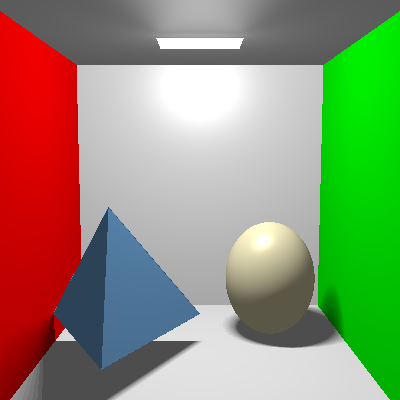
\includegraphics[width=4cm,height=5cm]{result_without_anti-aliasing}
	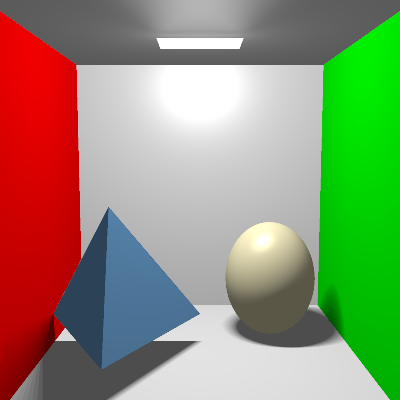
\includegraphics[width=4cm,height=5cm]{result_with_anti-aliasing}
	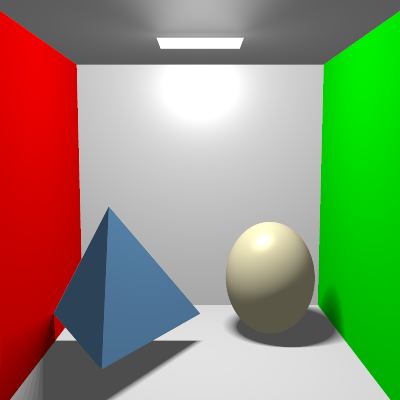
\includegraphics[width=4cm,height=5cm]{result_with_more_anti-aliasing}
	\caption{ray tracing to generate a graph, and compare the effects of anti-aliasing}
\end{figure}

\begin{figure}[h]
	\centering
	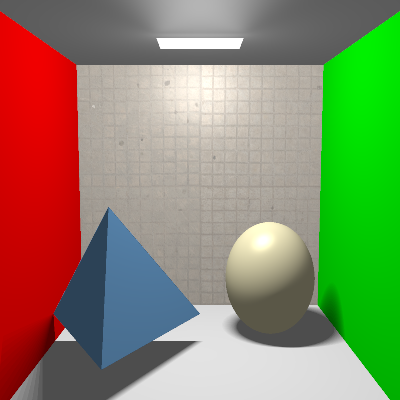
\includegraphics[width=4cm,height=5cm]{texture_mapping}
	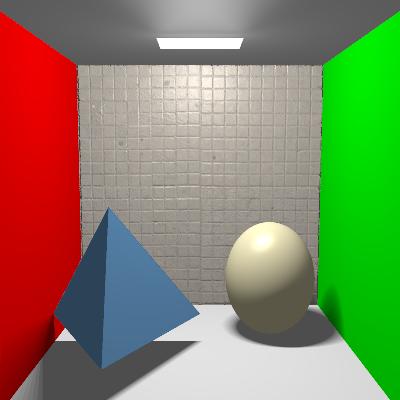
\includegraphics[width=4cm,height=5cm]{texture_normal_displacement}
	\caption{texture mapping}
\end{figure}

\begin{figure}[h]
	\centering
	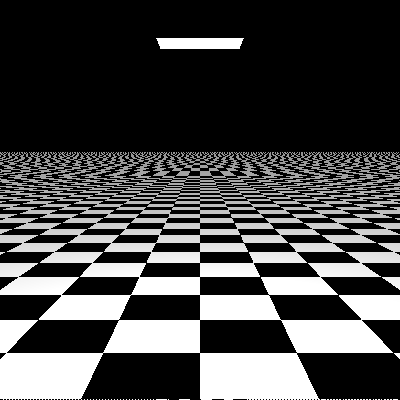
\includegraphics[width=4cm,height=5cm]{gird-simple}
	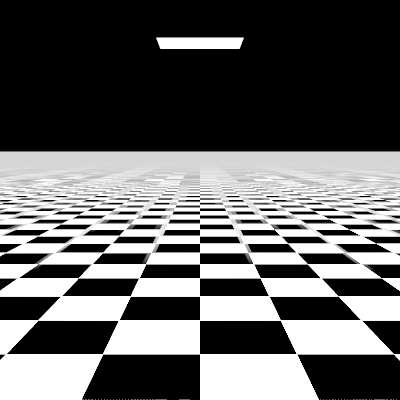
\includegraphics[width=4cm,height=5cm]{mip-map}
	\caption{texture filtering using mip-map}
\end{figure}

\begin{figure}[h]
	\centering
	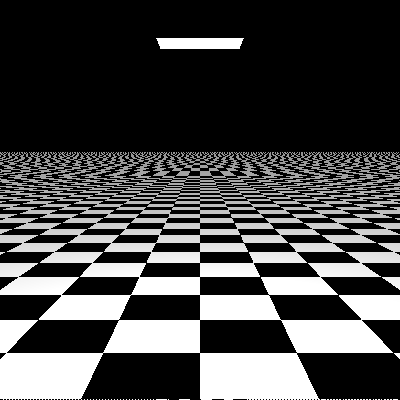
\includegraphics[width=4cm,height=5cm]{gird-simple}
	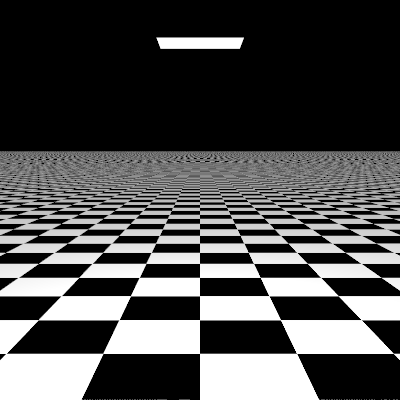
\includegraphics[width=4cm,height=5cm]{grid-multisample}
	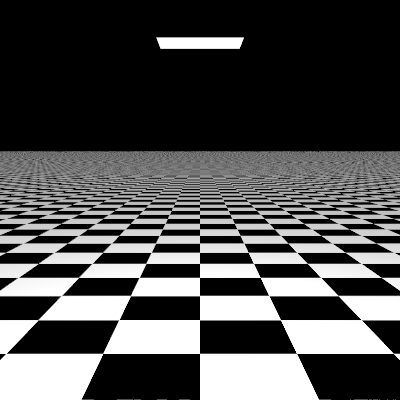
\includegraphics[width=4cm,height=5cm]{clockwise_rotation26.6}
	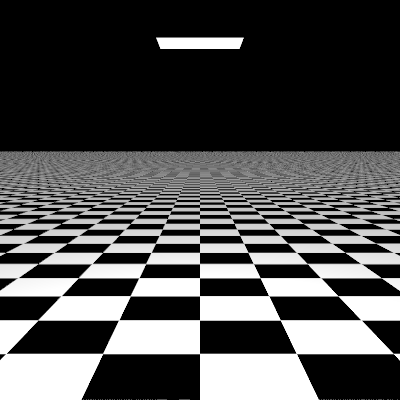
\includegraphics[width=4cm,height=5cm]{counter_clockwise_rotation26.6}
	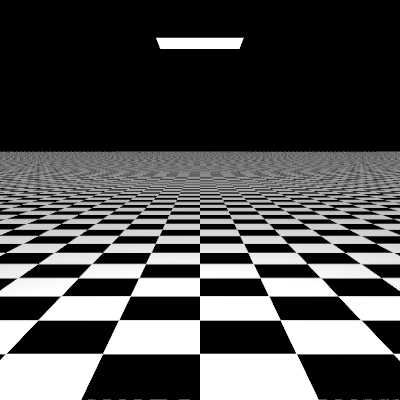
\includegraphics[width=4cm,height=5cm]{random_sample}
	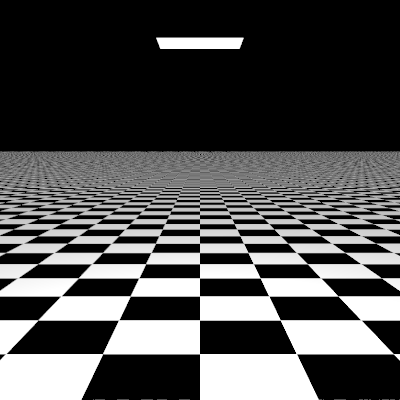
\includegraphics[width=4cm,height=5cm]{stratified_random_sample}
	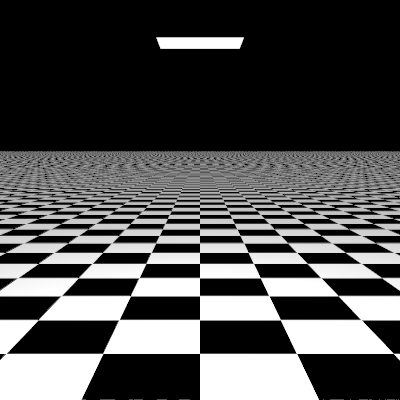
\includegraphics[width=4cm,height=5cm]{Halton}
	\caption{advanced anti-aliasing}
\end{figure}

\end{document}
